%%%%%%%%%%%%%%%%%%%%%%%%%%%%%%%%%%%%%%%%%%%%%%%%%%%%%%%
%% Engineer & Master Thesis, LaTeX Template          %%
%% Copyleft by Piotr Woźniak & Artur M. Brodzki      %%
%% Faculty of Electronics and Information Technology %%
%% Warsaw University of Technology, Warsaw, 2019     %%
%%%%%%%%%%%%%%%%%%%%%%%%%%%%%%%%%%%%%%%%%%%%%%%%%%%%%%%

\documentclass[
    left=2.5cm,         % Sadly, generic margin parameter
    right=2.5cm,        % doesnt't work, as it is
    top=2.5cm,          % superseded by more specific
    bottom=3cm,         % left...bottom parameters.
    bindingoffset=6mm,  % Optional binding offset.
    nohyphenation=true % You may turn off hyphenation, if don't like. =false
]{eiti/eiti-thesis} % bazuje na clasie mwart


%\usepackage[
%    backend=bibtex,
%    style=ieee
%]{biblatex}
\usepackage{csquotes}

\langpol % Dla języka angielskiego mamy \langeng
\graphicspath{{img/}}             % Katalog z obrazkami.
%\addbibresource{bibliografia.bib} % Plik .bib z bibliografią

% dodanie kropki po numerze w~LoL https://tex.stackexchange.com/questions/597350/add-dot-after-number-of-listing-in-list-of-listings
\makeatletter
\xpatchcmd\lst@MakeCaption{\protect\numberline{\thelstlisting}\lst@@caption}{\protect\numberline{\thelstlisting.}\lst@@caption}{}{}
%\makeatother
%\makeatletter
%\xpatchcmd{\LT@c@ption}{\protect\numberline{\thetable}}{\protect\numberline.{. \thetable . }}{}{}
\makeatother

\begin{document}

%--------------------------------------
% Strona tytułowa
%--------------------------------------
%\MasterThesis % dla pracy inżynierskiej mamy, tutaj praca koncowa
\EngineerThesis
\instytut{Telekomunikacji}

\title{
    Projekt i wdrożenie systemu bezpieczeństwa \\ 
    sieciowego w środowisku lokalnym z \\
    wykorzystaniem konteneryzacji \\
    wersja 05.2025
}

\engtitle{ % Tytuł po angielsku do angielskiego streszczenia
    Design and Implementation of a Network Security \\
    System in a Local Environment \\ 
    Using Containerization
}

\author{Łukasz Dejko (1203175)}

\promotor{dr inz. Jędrzej Bieniasz}

\date{\the\year}
\maketitle

%--------------------------------------
% Streszczenie po polsku
%--------------------------------------
\streszczenie Celem niniejszej pracy jest zaprojektowanie, wdrożenie oraz omówienie funkcjonalności kompleksowego systemu bezpieczeństwa sieciowego w środowisku lokalnym. System ten integruje mechanizmy ochrony warstwy DNS, filtrowanie ruchu HTTP, monitorowanie aktywności sieciowej, detekcję zagrożeń w czasie rzeczywistym oraz centralne gromadzenie i wizualizację danych telemetrycznych. Kluczowym założeniem projektu było wykorzystanie otwartoźródłowego oprogramowania oraz konteneryzacja usług przy użyciu platformy Docker, co zapewnia modularność, izolację oraz możliwość łatwego zarządzania środowiskiem.

Zastosowane komponenty umożliwiają kontrolę nad dostępem do sieci, blokowanie podejrzanych domen, analizę pakietów w czasie rzeczywistym oraz monitorowanie stanu systemu i usług. W pracy szczegółowo opisano konfigurację elementów odpowiedzialnych za filtrowanie DNS, wykrywanie intruzów, analizę logów oraz ich prezentację w formie czytelnych wykresów i pulpitów zarządczych. System został uruchomiony na serwerze domowym z systemem Linux oraz dodatkowo na platformie Raspberry Pi, co pokazuje elastyczność rozwiązania.

Projekt udowadnia, że także w warunkach domowych możliwe jest wdrożenie systemu bezpieczeństwa opartego na najlepszych praktykach znanych z infrastruktury korporacyjnej. Przedstawione podejście może stanowić punkt wyjścia do dalszych rozważań na temat bezpieczeństwa rozproszonych środowisk cyfrowych oraz implementacji polityk bezpieczeństwa opartych na danych telemetrycznych i analizie zagrożeń.

\slowakluczowe bezpieczeństwo sieci, DNS, Docker, analiza logów, filtracja treści, detekcja zagrożeń, Raspberry Pi, monitoring systemu

\newpage

%--------------------------------------
% Streszczenie po angielsku
%--------------------------------------
\abstract The purpose of this thesis is to design, implement, and analyze a comprehensive local network security system that integrates DNS-layer protection, HTTP traffic filtering, real-time network activity monitoring, threat detection, and centralized telemetry data visualization. A key objective of the project was the exclusive use of open-source software and containerization via the Docker platform, enabling modularity, service isolation, and ease of management across a distributed architecture.

The implemented solution allows full control over network access, blocking of suspicious domains, real-time traffic analysis, and detailed monitoring of system and service health. The thesis outlines the configuration of components responsible for DNS filtering, intrusion detection, log collection, and interactive dashboards. The system runs on a Linux-based home server and Raspberry Pi, demonstrating its adaptability and cost efficiency.

This work demonstrates that enterprise-grade security practices can be effectively replicated in a domestic setting using widely available technologies. The proposed solution can serve as a starting point for exploring secure digital environments and implementing policy-driven security based on telemetry data and behavioral threat analytics.
\keywords network security, DNS, Docker, log analysis, content filtering, threat detection, Raspberry Pi, system monitoring
\newpage

%--------------------------------------
% Oświadczenie o autorstwie
%--------------------------------------
%\makeauthorship
%\blankpage

%--------------------------------------
% Spis treści
%--------------------------------------
\thispagestyle{empty}
\tableofcontents
%\blankpage

%--------------------------------------
% Rozdziały
%--------------------------------------
\newpage 
\section{Wstęp}
\subsection{Cel pracy}

Głównym celem niniejszej pracy jest zaprojektowanie i wdrożenie kompleksowego systemu bezpieczeństwa sieciowego w środowisku lokalnym z wykorzystaniem konteneryzacji. System ma za zadanie nie tylko filtrować i kontrolować ruch sieciowy, lecz również analizować logi, wykrywać anomalie oraz umożliwiać monitorowanie stanu zasobów w czasie rzeczywistym.

Projekt zakłada integrację wielu niezależnych komponentów bezpieczeństwa opartych na oprogramowaniu typu open source. Do najważniejszych należą: lokalny serwer DNS z funkcją filtrowania (Pi-hole z Unbound), serwer proxy (Squid), system wykrywania zagrożeń IDS (Suricata), platforma do centralnego logowania i analizy zdarzeń (Graylog), system monitoringu (Prometheus i Grafana), a także konteneryzowane środowisko przeglądarki (Firefox) i narzędzia do zarządzania kontenerami (Portainer).

Celem pośrednim pracy jest także przedstawienie zalet architektury opartej na Dockera, takich jak elastyczność, skalowalność i separacja usług, oraz zastosowanie zasad bezpieczeństwa sieciowego w praktyce, w tym kontrola portów, firewall oraz zabezpieczenia hosta. Projekt ten stanowi dowód na to, że przy użyciu powszechnie dostępnych narzędzi można stworzyć bezpieczne i profesjonalne środowisko do zarządzania ruchem w sieci domowej lub małej firmie.

\subsection{Uzasadnienie wyboru tematu}

W dobie powszechnej cyfryzacji oraz rosnącej liczby zagrożeń związanych z bezpieczeństwem informacji, istotne staje się zapewnienie odpowiedniego poziomu ochrony nie tylko w środowiskach korporacyjnych, ale także w sieciach domowych. Coraz większa liczba urządzeń podłączonych do Internetu, takich jak smartfony, komputery, kamery IP czy inteligentne sprzęty AGD, powoduje zwiększoną ekspozycję na ataki z zewnątrz. Jednocześnie użytkownicy domowi często nie dysponują narzędziami ani wiedzą pozwalającą na skuteczne przeciwdziałanie zagrożeniom.

Wybór tematu pracy został podyktowany chęcią stworzenia systemu, który — bazując na darmowym oprogramowaniu i dostępnych komponentach sprzętowych — umożliwia wdrożenie rozwiązań znanych z profesjonalnych środowisk bezpieczeństwa IT. Zastosowanie takich narzędzi jak Pi-hole, Suricata czy Graylog pozwala na uzyskanie pełnej widoczności w ruchu sieciowym, detekcję podejrzanych aktywności oraz aktywne zarządzanie zagrożeniami w czasie rzeczywistym.

Temat pracy jest również odpowiedzią na potrzebę edukacji w zakresie budowy bezpiecznych środowisk informatycznych oraz wdrażania dobrych praktyk cyberbezpieczeństwa w ujęciu praktycznym. Dzięki konteneryzacji z użyciem Dockera możliwe jest szybkie i modularne wdrażanie usług, co znacząco ułatwia testowanie oraz skalowanie środowiska. Praca ta stanowi dowód na to, że budowa nowoczesnej i bezpiecznej sieci może być osiągalna nawet w warunkach ograniczonych zasobów.

\subsection{Zakres i ograniczenia pracy}

Zakres pracy obejmuje zaprojektowanie oraz wdrożenie zintegrowanego systemu bezpieczeństwa sieciowego w środowisku lokalnym z wykorzystaniem otwartoźródłowych narzędzi. Główne obszary realizacji obejmują: filtrowanie DNS i HTTP, wykrywanie anomalii w ruchu sieciowym, analizę i centralizację logów, monitoring systemów oraz zarządzanie kontenerami. Wszystkie usługi zostały uruchomione w kontenerach Docker, z wyjątkiem komponentów systemowych takich jak firewall czy Filebeat, które działają bezpośrednio na hoście.

Praca zawiera szczegółowy opis konfiguracji następujących komponentów:
\begin{itemize}
    \item serwera DNS z filtrowaniem (Pi-hole) oraz rekurencyjnego resolvera (Unbound),
    \item serwera proxy (Squid),
    \item systemu IDS (Suricata),
    \item platformy do analizy logów (Graylog, Elasticsearch, MongoDB),
    \item systemu monitoringu (Prometheus, Grafana),
    \item izolowanego środowiska przeglądarki (Firefox w kontenerze),
    \item systemu zarządzania kontenerami (Portainer),
    \item zapory sieciowej (iptables + ufw).
\end{itemize}

Ze względu na charakter projektu oraz ograniczone zasoby sprzętowe i czasowe, praca nie obejmuje testów penetracyjnych, implementacji systemów klasy EDR, ani automatycznych mechanizmów reakcji na incydenty. Projekt skupia się wyłącznie na rozwiązaniach dostępnych lokalnie — bez użycia usług chmurowych. Ponadto, wdrożone rozwiązania nie były poddawane audytowi zewnętrznemu, a skuteczność ich działania oceniana jest na podstawie obserwacji i dostępnych metryk.

Celem pracy nie jest stworzenie w pełni zgodnego z normami ISO środowiska bezpieczeństwa, lecz raczej przedstawienie możliwości zastosowania ogólnodostępnych narzędzi w celu zwiększenia poziomu ochrony danych i usług w domowej lub małej firmowej sieci komputerowej.

\subsection{Metodyka realizacji projektu}

Projekt został zrealizowany zgodnie z podejściem iteracyjnym, z podziałem na kolejne etapy obejmujące analizę wymagań, projektowanie architektury, konfigurację środowiska, wdrożenie usług, testowanie oraz dokumentację. Każdy z komponentów bezpieczeństwa został wdrażany i testowany niezależnie, a następnie integrowany z pozostałymi elementami w ramach jednej, spójnej infrastruktury kontenerowej.

Prace rozpoczęto od analizy możliwości sprzętowych oraz wyboru otwartoźródłowych narzędzi najlepiej odpowiadających założonym celom funkcjonalnym. Następnie zaprojektowano architekturę logiczną środowiska, w której istotne znaczenie miała separacja usług w kontenerach Docker i ich komunikacja przez dedykowane sieci wirtualne.

W kolejnych krokach skonfigurowano poszczególne komponenty systemu: serwery DNS, serwer proxy, system IDS, agregator logów oraz mechanizmy monitorujące. W celu zapewnienia spójności, dla każdej usługi utworzono oddzielne pliki konfiguracyjne oraz definicje kontenerów (Docker Compose). Równolegle prowadzono testy funkcjonalne poszczególnych modułów, weryfikując poprawność działania filtracji, detekcji i logowania zdarzeń.

Metodyka pracy zakładała również zastosowanie dokumentacji oficjalnej (ang. vendor documentation) oraz materiałów ogólnodostępnych, takich jak fora społecznościowe, blogi techniczne czy artykuły naukowe. W celu oceny skuteczności wdrożonych mechanizmów wykorzystywano dane z logów systemowych oraz panele monitorujące (dashboardy) stworzone w Grafanie i Graylogu.

Całość środowiska została osadzona na serwerze z systemem Debian oraz Raspberry Pi, co pozwoliło na weryfikację działania systemu zarówno w warunkach zasobooszczędnych, jak i przy większej wydajności. Projekt zrealizowano w środowisku domowym, co podkreśla jego dostępność i możliwość zastosowania w rzeczywistych warunkach.

\newpage 
\section{Opis środowiska i architektury systemu}
\subsection{Wykorzystany sprzęt i platforma systemowa}

Do realizacji projektu wybrano sprzęt, który zapewnia zarówno wysoką wydajność, jak i energooszczędność, co czyni go idealnym rozwiązaniem dla środowiska typu home lab. Główną jednostką obliczeniową jest komputer jednopłytkowy \textbf{Raspberry Pi 5} wyposażony w \textbf{8~GB pamięci RAM}. Jego najnowsza generacja charakteryzuje się znaczącym wzrostem mocy obliczeniowej względem poprzednich modeli, dzięki ulepszonemu procesorowi i zintegrowanemu układowi graficznemu. Taka konfiguracja pozwala na równoczesne uruchomienie wielu usług, takich jak \textit{Pi-hole}, \textit{Unbound}, \textit{Suricata} oraz \textit{Graylog}, bez zauważalnego spadku wydajności — nawet przy zwiększonym natężeniu ruchu sieciowego.

Jedną z kluczowych cech Raspberry Pi 5 jest obecność magistrali \textbf{PCIe}, która została wykorzystana do podłączenia dysku \textbf{NVMe Samsung SSD 980 o pojemności 500~GB}. Zastosowanie nośnika SSD w standardzie NVMe znacznie przyspieszyło operacje zapisu i odczytu danych w porównaniu do tradycyjnych kart microSD, co ma szczególne znaczenie w kontekście gromadzenia logów i działania systemów monitorujących.

Całość została umieszczona w dedykowanej obudowie \textbf{Argon NEO 5 M.2 NVMe PCIe}, która nie tylko zapewnia pasywne chłodzenie układów elektronicznych, ale również wspiera bezpośrednie mocowanie i integrację dysku SSD w formacie M.2. Obudowa została wykonana z aluminium, co przekłada się na wysoką trwałość oraz efektywne odprowadzanie ciepła, dzięki czemu możliwa jest długotrwała praca systemu bez ryzyka przegrzania. Kompaktowa forma oraz estetyczne wykonanie sprawiają, że zestaw doskonale wpisuje się w warunki domowego laboratorium.

Platforma systemowa oparta została na systemie \textbf{Raspberry Pi OS Lite}, będącym oficjalną dystrybucją Linuxa wspieraną przez Fundację Raspberry Pi. System ten zapewnia kompatybilność ze środowiskiem Docker oraz dostęp do bogatego repozytorium pakietów, co znacząco ułatwia wdrażanie usług kontenerowych. Wszystkie kontenery zostały uruchomione na silniku \textbf{Docker Engine} w wersji zgodnej z architekturą ARM64, natomiast ich zarządzanie odbywa się za pośrednictwem \textit{Portainera}.

Taka konfiguracja sprzętowo-programowa spełnia wymagania wydajnościowe i funkcjonalne projektu, zapewniając jednocześnie niski pobór mocy, cichą pracę i wysoką stabilność w warunkach domowych.

\subsection{Wirtualizacja i konteneryzacja (Docker + Portainer)}

W ramach niniejszego projektu zdecydowano się na wykorzystanie lekkiej formy wirtualizacji, jaką jest konteneryzacja z użyciem platformy Docker. Rozwiązanie to zostało wybrane ze względu na swoją elastyczność, wysoką wydajność oraz szerokie wsparcie społeczności i dostawców narzędzi open-source. Konteneryzacja umożliwia uruchamianie wielu odseparowanych usług w ramach jednego systemu operacyjnego, bez konieczności tworzenia pełnych maszyn wirtualnych. Dzięki temu znacznie redukowane są koszty zasobów oraz czas potrzebny na wdrożenie i zarządzanie poszczególnymi komponentami systemu bezpieczeństwa.

\textbf{Docker} pozwala na budowanie i uruchamianie aplikacji w formie kontenerów, które zawierają wszystkie niezbędne zależności — biblioteki, pliki konfiguracyjne oraz kod aplikacyjny. Każdy komponent systemu bezpieczeństwa (np. \textit{Pi-hole}, \textit{Unbound}, \textit{Suricata}, \textit{Graylog}, \textit{Prometheus}, \textit{Grafana}) został umieszczony w osobnym kontenerze, co znacząco zwiększa modularność i ułatwia konserwację systemu. Dodatkowo, każda usługa uruchamiana jest w odrębnej sieci wirtualnej Dockera, co umożliwia precyzyjne kontrolowanie ruchu sieciowego między kontenerami i hostem oraz zwiększa bezpieczeństwo całego środowiska.

Konfiguracja kontenerów została zautomatyzowana przy użyciu pliku \texttt{docker-compose.yml}, który umożliwia definiowanie całego stosu usług oraz ich zależności w sposób przejrzysty i powtarzalny. Taka forma zarządzania konfiguracją ułatwia proces wdrożenia oraz odtwarzania środowiska na innych urządzeniach lub po awarii.

W celu ułatwienia zarządzania środowiskiem kontenerowym wykorzystano narzędzie \textbf{Portainer} — graficzny interfejs użytkownika do zarządzania instancjami Docker. Portainer pozwala na monitorowanie kontenerów, wolumenów, obrazów, sieci oraz logów systemowych w czasie rzeczywistym. Dzięki niemu możliwe jest również szybkie uruchamianie i restartowanie usług, tworzenie nowych środowisk oraz kontrola nad dostępem użytkowników. Interfejs Portainera został zabezpieczony autoryzacją z hasłem i ograniczonym dostępem po porcie TCP/HTTPS, co stanowi dodatkowy element ochrony.

Separacja usług w kontenerach umożliwia niezależne zarządzanie i aktualizację każdego komponentu bez wpływu na pozostałe elementy systemu. Jest to szczególnie istotne w kontekście bezpieczeństwa: w przypadku wykrycia podatności w jednej z aplikacji, możliwe jest szybkie zastosowanie aktualizacji tylko dla konkretnego kontenera bez konieczności przerywania działania całego systemu.

Z punktu widzenia cyberbezpieczeństwa, konteneryzacja oferuje dodatkową warstwę izolacji procesów, co utrudnia eskalację uprawnień w przypadku ewentualnego włamania. Zastosowanie polityk sieciowych Dockera pozwala ograniczyć komunikację pomiędzy usługami tylko do niezbędnych przypadków, zgodnie z zasadą najmniejszych uprawnień (ang. \textit{principle of least privilege}).

Dzięki konteneryzacji cały system jest przenośny, łatwo skalowalny i podatny na automatyzację. Możliwe jest również wykorzystanie narzędzi takich jak \textit{Watchtower} do automatycznego aktualizowania kontenerów, co dodatkowo zwiększa poziom bezpieczeństwa systemu poprzez ograniczenie ekspozycji na znane podatności.

Podsumowując, zastosowanie Dockera i Portainera pozwoliło na stworzenie spójnego, modularnego i łatwego w utrzymaniu środowiska, które może być rozwijane i skalowane w przyszłości bez konieczności przebudowy całej infrastruktury.

\subsection{Architektura logiczna systemu bezpieczeństwa}
Architektura logiczna wdrożonego systemu bezpieczeństwa opiera się na centralnym serwerze zbudowanym na platformie Raspberry Pi 5, który pełni funkcję węzła integrującego różne usługi odpowiedzialne za filtrowanie, monitorowanie, analizę i kontrolę ruchu sieciowego w sieci lokalnej. Każdy komponent został uruchomiony w osobnym kontenerze Docker, co zapewnia ich niezależność oraz ułatwia aktualizację i zarządzanie.

Urządzenia końcowe w sieci domowej (komputery, smartfony, tablety, telewizory smart) komunikują się z Internetem poprzez serwer DNS realizowany przez \textbf{Pi-hole}. Serwer ten odpowiada za filtrowanie zapytań DNS i blokowanie niepożądanych domen (np. reklamowych, śledzących, złośliwych). Następnie zapytania DNS są przekazywane do \textbf{Unbound}, który jako rekurencyjny resolver zapewnia prywatność i niezależność od zewnętrznych dostawców DNS.

W celu kontroli dostępu do zasobów HTTP/S w Internecie ruch może być przekierowany przez serwer \textbf{Squid Proxy}, który dodatkowo umożliwia buforowanie i analizę treści. \textbf{Suricata} działa jako system detekcji i prewencji intruzów (IDS/IPS), analizując pakiety sieciowe w czasie rzeczywistym i wykrywając potencjalne zagrożenia na podstawie sygnatur oraz heurystyki.

Dane z logów zbierane są za pomocą \textbf{Filebeat} i kierowane do systemu \textbf{Graylog}, który umożliwia ich centralną analizę, przeszukiwanie i korelację. Jednocześnie, metryki systemowe i wydajnościowe są rejestrowane przez \textbf{Prometheus}, a ich wizualizacja odbywa się w \textbf{Grafanie} poprzez interaktywne dashboardy. Całe środowisko kontenerowe zarządzane jest z poziomu \textbf{Portainera}.

Wszystkie komponenty są połączone za pomocą wewnętrznych sieci wirtualnych Dockera, co ogranicza dostęp z zewnątrz do tylko niezbędnych portów i usług. Dzięki temu możliwe jest wdrożenie polityk bezpieczeństwa i izolacji na poziomie kontenerów. 

% Na rysunku~\ref{fig:architektura} przedstawiono uproszczony schemat logiczny systemu bezpieczeństwa.

% \begin{figure}[H]
%     \centering
%     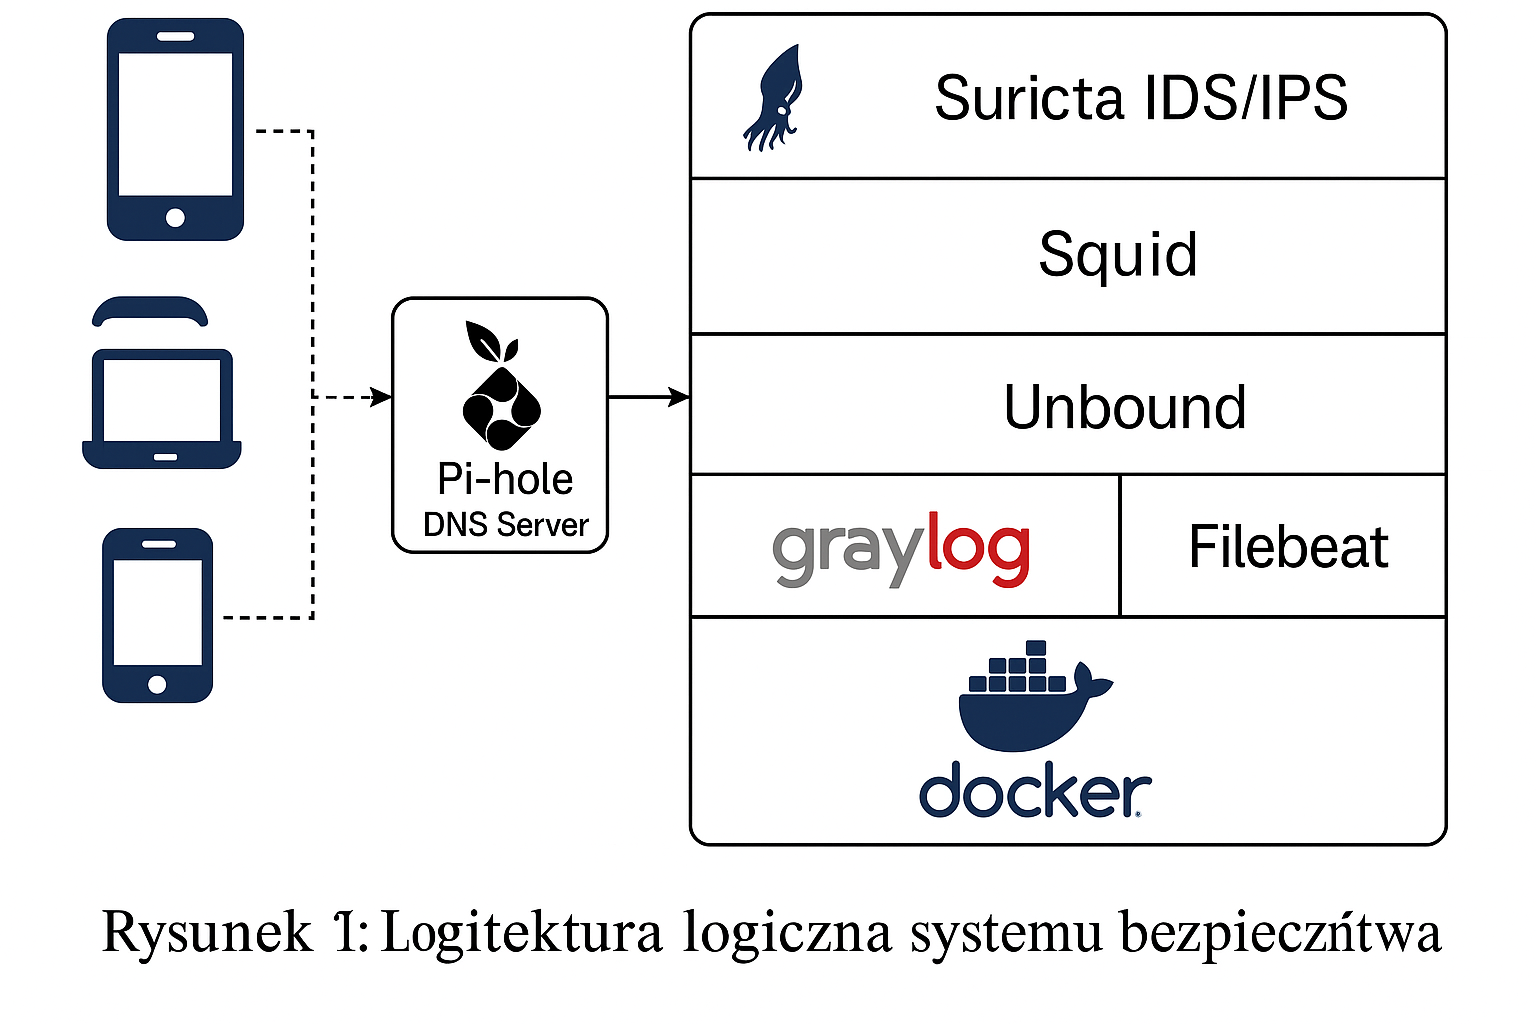
\includegraphics[width=0.95\textwidth]{A_diagram_illustrates_the_logical_architecture_of_.png}
%     \caption{Architektura logiczna systemu bezpieczeństwa}
%     \label{fig:architektura}
% \end{figure}

\subsection{Segmentacja i separacja usług w sieci lokalnej}

Jednym z kluczowych założeń projektowych było zapewnienie logicznej i funkcjonalnej separacji usług działających w ramach systemu bezpieczeństwa, co przekłada się bezpośrednio na podniesienie poziomu ochrony sieci lokalnej. Zastosowano podejście zgodne z zasadą \textit{security by design}, w którym każda usługa posiada wyraźnie zdefiniowaną funkcję, dostęp do tylko niezbędnych zasobów oraz ograniczoną komunikację z innymi komponentami.

Cała architektura została oparta na platformie Docker, która umożliwia uruchamianie poszczególnych usług w izolowanych kontenerach. Kontenery te zostały pogrupowane w logiczne segmenty sieci wirtualnych Docker, co pozwala na granularne kontrolowanie komunikacji między nimi. Przykładowo, kontener \textit{Squid Proxy} ma dostęp do zewnętrznego Internetu oraz do kontenerów \textit{Pi-hole} i \textit{Unbound}, lecz nie posiada bezpośredniego połączenia z usługami logującymi, takimi jak \textit{Graylog} czy \textit{Prometheus}.

Separacja realizowana jest również na poziomie warstwy sieciowej dzięki wykorzystaniu wielu mostów sieciowych (ang. \textit{Docker bridge networks}). Dla każdej grupy usług zdefiniowano osobną sieć wirtualną, co pozwala na kontrolowanie tras routingu, zamykanie nieużywanych portów oraz precyzyjne definiowanie reguł dostępu przy użyciu mechanizmów zapory ogniowej (iptables) oraz konfiguracji Dockera.

Z poziomu systemu hosta (Raspberry Pi 5), zastosowano dodatkowe zabezpieczenia w postaci lokalnego firewalla (ufw), który ogranicza dostęp do wybranych portów wyłącznie z określonych adresów IP lub interfejsów sieciowych. Dzięki temu dostęp do interfejsów zarządzających (np. Portainer, Graylog, Grafana) możliwy jest wyłącznie z wybranych urządzeń w sieci lokalnej, co znacząco ogranicza powierzchnię potencjalnych ataków.

Dodatkowo, każda aplikacja kontenerowa uruchamiana jest z jak najmniejszym zestawem uprawnień (zgodnie z zasadą najmniejszych przywilejów), bez trybu uprzywilejowanego (ang. \textit{--privileged}) oraz bez montowania niepotrzebnych wolumenów hosta. W miejscach wymagających zapisu danych (np. logi, konfiguracje), wykorzystano dedykowane wolumeny Docker z ograniczonym dostępem do systemu plików.

Segmentacja logiczna i funkcjonalna usług nie tylko zwiększa bezpieczeństwo, ale również ułatwia zarządzanie systemem, umożliwia szybsze diagnozowanie problemów oraz ogranicza skutki ewentualnych błędów lub kompromitacji poszczególnych komponentów. Rozdzielenie usług umożliwia też niezależne aktualizacje i restarty bez wpływu na stabilność całego środowiska.

\newpage 
\section{Konfiguracja i rola poszczególnych komponentów}
\subsection{Pi-hole jako centralny DNS filtrujący}

\textbf{Pi-hole} pełni w prezentowanym systemie funkcję centralnego serwera DNS, odpowiadającego za obsługę zapytań DNS z całej sieci lokalnej. Jego głównym zadaniem jest filtrowanie niechcianych zapytań do domen z list czarnej listy (blacklist), w tym blokowanie reklam, śledzenia użytkowników (trackery), elementów malware oraz innych potencjalnie niebezpiecznych domen. Dzięki temu Pi-hole stanowi pierwszą linię obrony przed wieloma zagrożeniami jeszcze zanim ruch opuści sieć lokalną.

Pi-hole został uruchomiony w kontenerze Docker na platformie Raspberry Pi 5, co umożliwia jego łatwą aktualizację, przenoszenie oraz niezależne zarządzanie. Kontener został skonfigurowany z odpowiednimi wolumenami trwałymi, umożliwiającymi zachowanie ustawień i statystyk po restarcie. W konfiguracji uwzględniono mapowanie portów 53 (UDP i TCP) dla zapytań DNS oraz port 80 dla interfejsu webowego, z dodatkowym ograniczeniem dostępu za pomocą firewalla.

Pi-hole został połączony z usługą \textbf{Unbound}, która działa jako lokalny, rekurencyjny resolver DNS. Taki układ eliminuje konieczność korzystania z zewnętrznych serwerów DNS (np. Google, Cloudflare), co znacząco poprawia prywatność użytkownika i uniezależnia system od komercyjnych operatorów. Zapytania rozwiązywane są bezpośrednio od źródła (root DNS servers), z wykorzystaniem mechanizmów weryfikacji DNSSEC.

Lista blokowanych domen oparta jest o popularne źródła publiczne, takie jak \texttt{https://firebog.net}, uzupełnione o ręcznie dodane wpisy dopasowane do potrzeb użytkowników domowych. Pi-hole rejestruje każde zapytanie DNS i udostępnia statystyki w czytelnej formie webowego interfejsu administracyjnego. Użytkownik może przeglądać historię zapytań, najczęściej blokowane domeny, statystyki według urządzeń, a także dynamicznie zarządzać listami dozwolonych (whitelist) i zablokowanych (blacklist) domen.

Dodatkowo skonfigurowano opcję logowania DNS w formacie syslog, co umożliwia przesyłanie logów do narzędzia \textbf{Filebeat}, a następnie do systemu analitycznego \textbf{Graylog}. Dzięki temu możliwe jest korelowanie zapytań DNS z innymi zdarzeniami w sieci oraz budowa dashboardów z wizualizacją aktywności DNS.

Z perspektywy bezpieczeństwa, Pi-hole pozwala na:
\begin{itemize}
    \item blokowanie phishingu i złośliwych domen,
    \item ograniczenie śledzenia przez zewnętrzne podmioty (trackery reklamowe),
    \item zwiększenie prywatności użytkowników sieci lokalnej,
    \item filtrowanie treści nieodpowiednich dla dzieci (przy odpowiedniej konfiguracji list).
\end{itemize}

W ramach systemu Pi-hole stanowi zatem kluczowy komponent w warstwie prewencji i kontroli ruchu DNS, a jego integracja z Unbound oraz systemami logującymi czyni go silnym narzędziem analityczno-filtrowym w domowej infrastrukturze bezpieczeństwa.

\subsection{Unbound jako rekurencyjny resolver DNS}

\textbf{Unbound} pełni w opisywanym systemie rolę lokalnego, rekurencyjnego resolvera DNS, który współpracuje bezpośrednio z serwerem Pi-hole. Jego głównym zadaniem jest niezależne i bezpieczne rozwiązywanie zapytań DNS, bez udziału zewnętrznych operatorów (takich jak Google DNS czy Cloudflare), co znacząco zwiększa poziom prywatności i integralności komunikacji sieciowej.

Zamiast przekazywać zapytania DNS dalej do publicznych resolverów, Unbound kontaktuje się bezpośrednio z autorytatywnymi serwerami DNS — począwszy od tzw. root servers — a następnie iteracyjnie pobiera odpowiedzi od serwerów nadrzędnych (TLD) aż do uzyskania odpowiedzi końcowej. Dzięki temu możliwe jest uniezależnienie infrastruktury od zewnętrznych dostawców oraz lepsza kontrola nad ruchem DNS.

W środowisku projektu Unbound został skonfigurowany jako osobny kontener Docker, z dostępem jedynie z wewnętrznej sieci Dockerowej, do której podłączony jest również kontener Pi-hole. W ten sposób zapytania DNS przychodzące od klientów trafiają najpierw do Pi-hole (który wykonuje filtrowanie), a następnie przekazywane są do Unbound w celu rekurencyjnego rozwiązania. Taka dwupoziomowa struktura poprawia zarówno bezpieczeństwo, jak i dokładność obsługi zapytań.

Konfiguracja Unbound została oparta na oficjalnych wytycznych projektu Pi-hole, z dodatkowymi usprawnieniami bezpieczeństwa:
\begin{itemize}
    \item włączono \textbf{DNSSEC} – mechanizm weryfikacji kryptograficznej odpowiedzi DNS,
    \item ograniczono maksymalną liczbę jednoczesnych klientów, aby zapobiec atakom DDoS,
    \item skonfigurowano Unbound do pracy tylko w trybie lokalnym, nasłuchującym jedynie na interfejsach wewnętrznych,
    \item ustawiono cache DNS w celu przyspieszenia odpowiedzi na często powtarzające się zapytania.
\end{itemize}

Dzięki zastosowaniu Unbound jako lokalnego resolvera możliwe jest osiągnięcie następujących korzyści:
\begin{itemize}
    \item pełna niezależność od zewnętrznych dostawców DNS,
    \item zwiększenie prywatności zapytań DNS (brak logowania i śledzenia przez operatorów zewnętrznych),
    \item wsparcie dla DNSSEC – ochrona przed zatruciem cache i fałszywymi odpowiedziami,
    \item skrócenie czasu odpowiedzi dzięki lokalnemu cache.
\end{itemize}

Współpraca Pi-hole z Unbound stanowi nowoczesne i bezpieczne rozwiązanie DNS, rekomendowane w środowiskach, gdzie priorytetem jest prywatność użytkownika, integralność danych oraz niezależność od usług zewnętrznych. Całość działa w pełni lokalnie, co jest istotne w kontekście koncepcji „zero trust” oraz ograniczania powierzchni ataku.

\subsection{Squid Proxy – filtrowanie i kontrola dostępu do Internetu}

\textbf{Squid Proxy} pełni w systemie funkcję transparentnego pośrednika w komunikacji HTTP i HTTPS pomiędzy urządzeniami końcowymi a zasobami Internetu. Jego zadaniem jest nie tylko buforowanie treści w celu przyspieszenia dostępu i ograniczenia ruchu wychodzącego, ale przede wszystkim implementacja reguł filtrowania, kontroli dostępu oraz logowania zdarzeń sieciowych w warstwie aplikacji.

W niniejszym projekcie Squid został uruchomiony jako osobny kontener w środowisku Docker, w ramach tej samej infrastruktury opartej na Raspberry Pi 5. Kontener został przydzielony do sieci wirtualnej wspólnej z kontenerem Pi-hole i Unbound, co umożliwia jego pełną integrację z warstwą DNS. Urządzenia końcowe w sieci lokalnej (komputery, smartfony, tablety) kierują ruch HTTP/S do Squida, który następnie rozwiązuje adresy DNS za pośrednictwem Pi-hole i Unbound, oraz przekazuje żądania dalej — do Internetu.

Konfiguracja Squida została dostosowana do potrzeb środowiska domowego, z naciskiem na bezpieczeństwo, przejrzystość i możliwość rozbudowy. Wdrożono następujące mechanizmy:
\begin{itemize}
    \item \textbf{ACL (Access Control Lists)} – listy kontroli dostępu definiujące, które adresy IP, domeny lub kategorie URL mogą być dostępne, a które blokowane,
    \item \textbf{Blokowanie treści niepożądanych} – filtrowanie stron zawierających reklamy, treści dla dorosłych lub znane z hostowania złośliwego oprogramowania,
    \item \textbf{Zarządzanie ruchem HTTPS} – obsługa połączeń TLS z pominięciem inspekcji pakietów, z zachowaniem logów statystycznych na poziomie domen,
    \item \textbf{Cache HTTP} – buforowanie często odwiedzanych zasobów w celu oszczędzania pasma i szybszego ładowania stron,
    \item \textbf{Transparent proxy} – możliwość pracy w trybie przeźroczystym, gdzie ruch przekierowywany jest automatycznie z poziomu routera/firewalla (w przyszłych wdrożeniach).
\end{itemize}

Wszystkie logi generowane przez Squida są kierowane do systemu \textbf{Filebeat}, a następnie przesyłane do \textbf{Grayloga}, gdzie podlegają korelacji z innymi zdarzeniami sieciowymi (np. alertami z Suricaty czy zapytaniami DNS). Dzięki temu możliwe jest śledzenie i analiza aktywności użytkowników oraz wykrywanie potencjalnych anomalii, takich jak próby dostępu do nieautoryzowanych serwisów, złośliwy ruch wychodzący czy wykorzystanie tuneli proxy.

Squid umożliwia również stworzenie podstawowych polityk kontroli dostępu do Internetu, takich jak:
\begin{itemize}
    \item ograniczenia czasowe (np. blokada serwisów społecznościowych poza godzinami pracy),
    \item białe i czarne listy domen lub kategorii treści,
    \item ograniczenia transferu danych dla konkretnych adresów IP lub grup.
\end{itemize}

Integracja Squida z Pi-hole i Unbound zapewnia spójność filtracji oraz centralizację zarządzania ruchem sieciowym. Całość działa wewnątrz odizolowanego środowiska Docker, co znacząco podnosi poziom bezpieczeństwa i pozwala łatwo wdrażać aktualizacje i rozszerzenia.

Podsumowując, Squid Proxy w tej architekturze pełni kluczową rolę w wymuszaniu polityk bezpieczeństwa, filtrowaniu treści oraz zapewnianiu przejrzystości działania użytkowników w sieci domowej.


\end{document}